\chapter{Experiments}\label{experiments}

The purpose of the application is to speed up the computation process,
thus it should be verified, whether the improvement makes sense or do
not. The improvement should correspond to the number of nodes involved
in the computation. What we wish is, that the dependence is of some
linear form, that is, the computation gets faster with every additional
node and it improves by the same steps. In this hypothetical ideal case
two nodes means two times faster computation and one hundred nodes means
one hundred times faster achievement of the result. However, this is
impossible for several reasons. At first, we must consider time that is
taken by the division process. More time is needed for transfers and
final join operation. Another problem raises because of the fact that
the transfers are quite demanding themselves so when more transfers are
ongoing at a particular moment, the initiator is more utilized and the
process could be slowed down due to this fact. This also implies that
the improvement does not raise constantly when adding more nodes.
Finally, we must consider that in the real situation delays can appear
due to technical reasons, network congestion or node failures.

\section{Aproach to testing}\label{aproach-to-testing}

If we want to obtain reasonable data, the measurements must be repeated
several times to prevent deviations. Also we want to keep the
measurements independent so its statistical processing is easier. Our
approach to running the tests and gathering results is described in this
chapter. Our main goal is to measure the improvement, but we would also
like to measure the impact the particular setting has on the result.

Because of the number of tests, it is desirable that the testing process
is automated. Because of that, special Bash script was used to run the
tests. The script is tailored to be used at the testing laboratory, so
it may need little modifications to work in some different environment.
It is distributed with the source code of the framework. To allow
automated and robust execution of the test, special functionality was
added to the program. It is invokable by option given at the start time
and causes the program to run in non-interactive mode, i.e.~keyboard
input is accepted, the program just processes given file and ends. This
options ?? all the essential data are given when the program is started.
To keep the measurements independent, all the instances (on every node)
of the program are started at the test beginning and they are killed in
the end. Communication with the remote nodes is handled by the ssh
program. The testing script uses a special file which describes the
particular run. Working example of such file together with explanations
of the values is given below.

\begin{samepage}
\begin{verbatim}
v6 // use IPv6
/afs/ms/u/h/hudecekv/futu.avi // location of the file to be re-encoded
2 // run the whole scenario twice
slower // quality of the encoding
10000 // chunk size [KByte]
2048576 // transfer buffer size
spawn u-pl1 2221 // spawn the program on the machine 'u-pl1', use port 2221
spawn u-pl2 2222
spawn u-pl4 2224
spawn u-pl5 2225
spawn u-pl6 2226
spawn u-pl7 2227
wait 10 // wait for ten seconds before next action
kill u-pl4 // kill the instance of program running on machine 'u-pl4'
spawn u-pl8 2228
spawn u-pl9 2229
spawn u-pl10 2230
\end{verbatim}
\end{samepage}

Thanks to this mechanism, various scenarios can be run easily without
the need of human interaction. The test data were collected by running
the test ten times for the given count of nodes. The count varied from
one to ten nodes involved. Each test was run once with chunks of 40 000
kB in size and once with 10 000 kB chunks. The same file was used each
time as well as the encoding quality. Each test stored various results,
among others the average times needed for transfer and encoding, number
of chunks, quality and count of involved nodes. Because we had not the
chance to run the tests in some dedicated network, the computation times
may vary for the given setting depending on the current conditions. The
tests showed however, that if we multiply the average time needed to
encode one chunk by the count of chunks, the product corresponds to the
time that would be taken by the normal encoding process. This allows us
to deal with the problem, because we can compare the time with this
computed estimation and the error will be minimal. The desired values
have been gathered in two ways. Some of them, for example average
transfer and encoding times, are measured directly in the program and
then outputted in special file. The script just reads it from this file.
The rest of the values is obtained in the script. \#\# Results
Measurings showed, that the dependence between the number of involved
nodes and the improvement is approximately logarithmic. To evaluate the
data, simple linear regression model was used. Specifically, subsequent
formula was used:

\begin{center}
$\frac{distributed\_time}{single_node_time} = x_1 \times log(neighbor_count - 0.9)$
\end{center}

The absolute value has been added since the model fits better this way -
in the case when one neighbor is used, the distributed computation is
actually slower. In the following figures are showed the achieved
results. The blue dashed line represents the estimate based on the
model. The data are visualized as black crosses, red squares show
respective mean values.

\begin{figure}[h]
\begin{center}
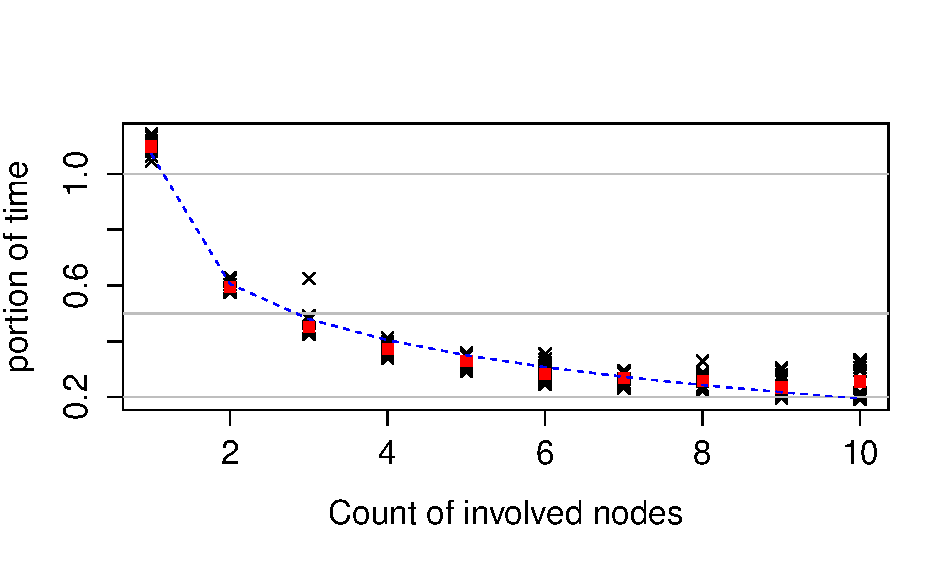
\includegraphics[scale=0.90]{./img/Rplot.pdf}
\caption{Achieved improvement - all measurements}
\end{center}
\end{figure}

\begin{figure}[h]
\begin{center}
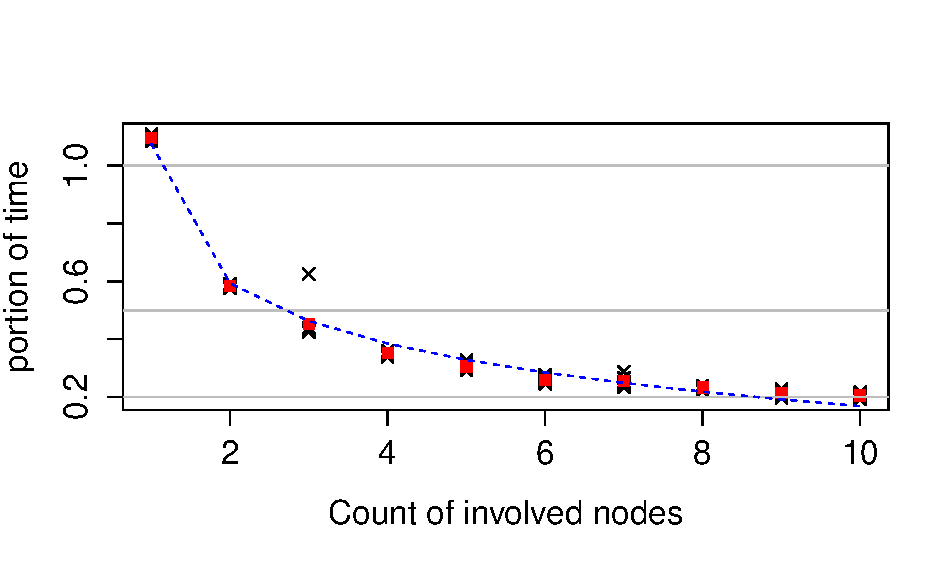
\includegraphics[scale=0.90]{./img/Rplot10k.pdf}
\caption{Achieved improvement - 10 MB chunks}
\end{center}
\end{figure}

\begin{figure}[h]
\begin{center}
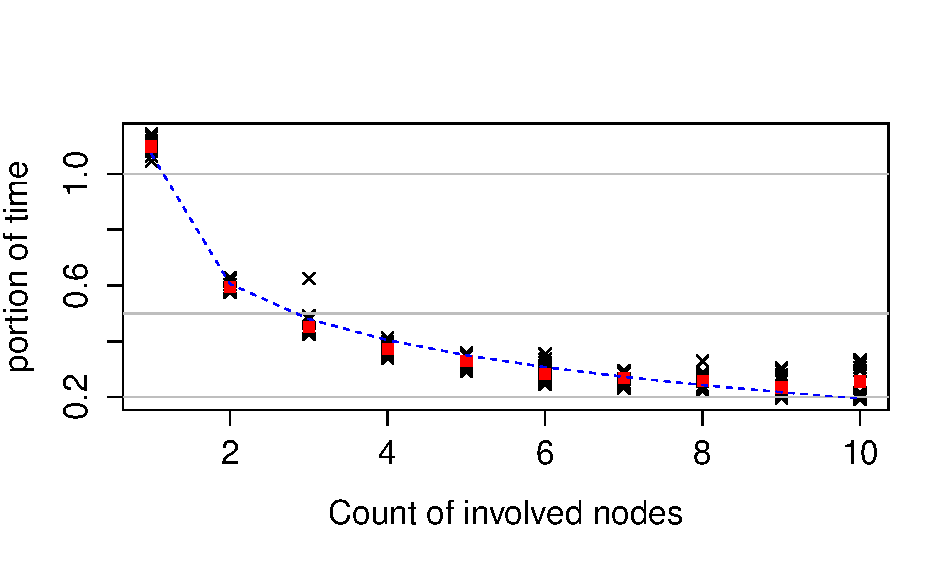
\includegraphics[scale=0.90]{./img/Rplot.pdf}
\caption{Achieved improvement - 40 MB chunks}
\end{center}
\end{figure}
